\begin{frame}[parent={cmap:software-testing-foundations}, hasprev=false, hasnext=true]
\frametitle{Defect}
\label{concept:defect}

\begin{block:fact}{Defective products}
\begin{itemize}
    \item No product is defect-free.
    \begin{itemize}
		\item And that applies to any kind of product, be it software or
		hardware.
    \end{itemize}
\end{itemize}

\hfill
\refie{example:product-failures}{\beamerbutton{Example: Product failures}}
\end{block:fact}


\begin{block:fact}{Defective software}
\begin{itemize}
	\item No software module is defect-free when implemented and only 40\% of
    software modules are defect-free when released~\cite{shull-etal:2002}.
\end{itemize}
\hfill
\refie{example:software-failures}{\beamerbutton{Example: Software failures}}
\end{block:fact}
\end{frame}


\begin{frame}[hasprev=true, hasnext=true]
\frametitle{Defect}
\label{concept:defect-detection}

\begin{block:fact}{Every software has defects}
\begin{itemize}
	\item Even small, simple, trivial products are error-prone.
\end{itemize}
\end{block:fact}

\begin{block}{Example: Triangle}
\centering
\refie{example:triangle}{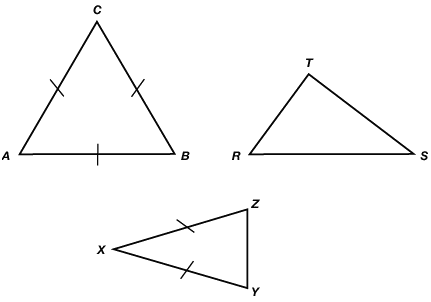
\includegraphics[scale=.5]{resources/Triangle/Equilateral-Isosceles-Scalene-triangles}}
\end{block}
\end{frame}


\begin{frame}[hasprev=true, hasnext=false]
\frametitle{Defect}

\begin{block:fact}{Defect avoidance and detection}
\begin{itemize}
	\item Nevertheless, products failures could and must be avoided and
	corrected, as they negatively impacts software quality.
\end{itemize}
\end{block:fact}


\begin{block:fact}{Why we should care about it?}
\begin{itemize}
    \item Rising demand for higher software quality.

    \item Software defect reduction improves software quality.
\end{itemize}
\end{block:fact}

\begin{block:fact}{Software quality and software testing}
\begin{itemize}
	\item The main goal of software testing is to find defects.

	\item Systematic software testing, carried out using proper techniques,
	criteria, and tools, improves software reliability (and quality).
\end{itemize}
\end{block:fact}
\end{frame}
